\documentclass{article}
\usepackage[utf8]{inputenc}
\usepackage{amsmath,amssymb}
\usepackage{graphicx}
\usepackage[a4paper,margin=1.2cm]{geometry}
\usepackage{multicol}
\graphicspath{ {./img/} }

\DeclareMathOperator{\ima}{Im}


\begin{document}

\section{Criteri di diagonalizzabilità (1° e 2°)}
\begin{itemize}
    \item una matrice di grado n deve avere n autovalori distinti
    \item la somma delle \(m_a\) è n e ogni autovalore è regolare (stessa molteplicità algebrica e geometrica)(\(m_g\)=null(A-\(\lambda\)I))
\end{itemize}

\section{Matrice modale e diagonale}
{\large Una volta verificato che la matrice è diagonalizzabile si possono trovare la matrice modale e la matrice diagonale tali che 
\( (M^{-1}AM=D) \)}
\begin{itemize}
    \item la matrice modale si crea usando gli autovettori come colonne
    \item la matrice diagonale si crea mettendo gli autovettori come elementi della diagonale
\end{itemize}

\section{Basi e coordinate}
Dati V spazio vettoriale di dimensione n e W spazio vettoriale di dimensione m\\
B base di V e B' base di W\\
T una trasformazione lineare T:V\(\rightarrow{}\)W\\\\
{\large A è la matrice tale che \(C_{B'}(T(v))=AC_{B}(v)\)}\\\\
La matrice A è la matrice rappresentativa della trasformazione lineare T nelle basi B e B'\\
\begin{center}
    \(M^{B'}_B(T)\)
\end{center}
\subsection{Calcolo della matrice rappresentativa}
La i-esima colonna di \(M^{B'}_B(T)\) è\\
\begin{center}
    \(M^{B'}_B(T)^i=C_{B'}(T(v_i))\)
\end{center}
\(M^{B'}_B(T)\) è la matrice che ha per i-esima colonna il vattore delle coordinate in B' dell'i-esimo elemento di B\\

\section{Prodotto scalare}

La norma di un vettore libero è la sua lunghezza
\begin{center}
v=x\(\vec{i}\)+y\(\vec{j}\)\\
\(\lvert\lvert\)v\(\rvert\rvert=\sqrt{x^2+y^2}\)
\end{center}
Distanza tra 2 punti (norma del vettore tra i due punti)
\begin{center}
    d(P,Q)=\(\lvert\lvert\vec{P}\vec{Q}\rvert\rvert=\sqrt{(x_1-x_0)^2+(y_1-y_0)^2}=\lvert\lvert x-x_0\vec{i}+y_1-y_0\vec{j}\rvert\rvert\)
\end{center}
\begin{center}
{\Large Prodotto scalare}
\[v\cdot w=\lvert\lvert v \rvert\rvert \cdot \lvert\lvert w \rvert\rvert \cdot \cos\theta\]
con \(\theta\) angolo minimo tra i due vettori
\end{center}
\begin{itemize}
    \item \(v\perp c \Leftrightarrow v \cdot w = 0\) (v è ortogonale a w se il prodotto scalare è 0)
    \item \(\lvert\lvert v \rvert\rvert = \sqrt{v \cdot v}\) (norma e prodotto scalare)
    \item \(d(PQ) = \lvert\lvert \vec{PQ}\rvert\rvert = \sqrt{\vec{PQ} \cdot \vec{PQ}}\) (distanza e prodotto scalare)
\end{itemize}
Espressione analitica del prodotto scalare\\\\
se \(v=x_1\vec{i} + y_1\vec{j}\) e \(w=x_2\vec{i} + y_2\vec{j}\) allora\\ 
\(v \cdot w = x_1 \cdot x_2 + y_1 \cdot y_2\)\\\\\\\\\\
Disuguaglianza di schwarz\\\\
se v e w sono due vettori in V\\
\(\lvert\lvert v \cdot w \rvert\rvert \leq \lvert\lvert v \rvert\rvert \cdot \lvert\lvert w \rvert\rvert\)\\\\\\ 
Disuguaglianza triangolare\\\\
se v e w sono due n-vettori\\
\(\lvert\lvert v + w \rvert\rvert \leq \lvert\lvert v \rvert\rvert + \lvert\lvert w \rvert\rvert\)\\\\\\ 
{\Large Proiezione ortogonale}\\\\
Dati due vettori liberi nel piano o nello spazio v e w\\
La proiezione ortogonale di v lungo il vettore w è \(P_w(v)\)\\
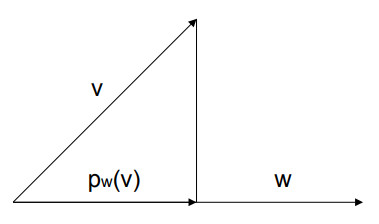
\includegraphics[scale=0.5]{prort.png}\\
Proprietà
\begin{itemize}
    \item \(P_w(v)\) ha la stessa direzione di w
    \item \(v - P_w(v)\) è ortogonale a w
\end{itemize}
\begin{center}
    {\large Calcolo della proiezione ortogonale}
\end{center}
\[P_w(v) = \frac{v\cdot w}{w\cdot w} w = \frac{v \cdot w}{\lvert\lvert w \rvert\rvert^2} w\]\\

\section{Basi ortonormali}
{\Large Insiemi ortogonali e ortonormali}\\\\
un insieme \{\(v_1,v_2,\ldots,v_k\)\} di vettori in uno spazio V
\begin{itemize}
    \item  è ortogonale se \(v_i\neq\vec{0}\)  \(\forall i\)   e \(v_i\cdot v_j = 0\) per \(i\neq j\)
    \item è ortornormale se \(\lvert\lvert v_i \rvert\rvert = 1 \forall i\)
\end{itemize}
\begin{center}
    {\large Da ortogonale a ortonormale}\\
    con \(\{v_1,v_1,\ldots,v_k\}\) ortogonale e \(\{w_1,w_1,\ldots,w_k\}\) ortonormale
    \[w_i=\frac{v_i}{\lvert\lvert v_i \rvert\rvert}\]
\end{center}
Gli insiemi ortogonali sono sempre linearmente indipendenti\\\\
{\large Come trovare una base ortonormale di uno spazio euclideo}\\
Ortonormalizzazione
\begin{enumerate}
    \item si sceglie una base B=\{\(v_1,v_2,\ldots,v_k\)\}
    \item si pone \(U_1=V_1\)
    \item poi \(U_2 = V_2 + \alpha U_1 \) tale che \(U_1 \cdot U_2 = 0\)
    \item poi si procede allo stesso modo con  \(U_3 = V_3 + \alpha U_1 + \beta U_2\) tale che \(U_1 \cdot U_2 = 0\) e \(U_1 \cdot U_3 = 0\)
\end{enumerate}
(si avrà un sistema di n incognite in base al numero di vettori della base (2 vettori, 1 incognita; 3 vettori, 2 incognite...))\\
Poi si normalizza \(\rightarrow{} w_i=\frac{U_i}{\lvert\lvert U_i \rvert\rvert}\)\\
\(\{w_1,w_2,\ldots,w_n\}\) è ortonormale
\begin{itemize}
    \item ///\\
\end{itemize}
{\large Matrici ortogonali}\\\\
Una matrice A è ortogonale se \\
\(A^T=A^-1 \leftrightarrow A^TA = I \leftrightarrow AA^T = I\)\\
La matrice è ortogonale se le sue colonne formano una base ortonormale\\\\

{\large Spazio ortogonale}\\\\
Sia U sottospazio di uno spazio euclideo V\\
\(U^\perp = \{v\in V | u \cdot v = 0 \forall u \in U\}\) è uno spazio vettoriale\\
\(U^\perp\) è complemento di U in V\\\\\\
{\large Spazio ortogonale di R(A)}\\\\
Si ha che \(R(A)^\perp = N(A^T)\)\\
Osservazione\\
Se U = R(A) allora \(U^\perp = R(A^T)\) (R(A) = spazio colonna)\\\\\\
B-espansione di un vettore\\\\
Se \(B= \{q_1,q_2,\ldots,q_n\}\) è una base ortonormale di uno spazio euclideo V e v è un vettore, allora,\\
\(v=(v\cdot q_1)q_1+\ldots+(v\cdot q_n)q_n\)    Questa è la B-espansione di v\\\\\\
Vettore delle coordinate in una base ortonormale\\\\
Se \(B=\{q_1,q_1,\ldots,q_n\}\) è una base ortonormale di uno spazio euclideo V allora il vettore delle coordinate di v nella base B è\\
\(C_B(V)=\left(
\begin{array}{c}
    v\cdot q_1 \\
    v\cdot q_2 \\
    \vdots     \\
    v\cdot q_n \\
\end{array}\right)\)\\\\\\\\
Matrice di una trasformazione lineare in una base ortonormale\\\\
Se V è uno spazio euclideo e \(T:V\rightarrow{}V\) trasformazione lineare allora la matrice di T in una base ortonormale B è data da\\
\(M_B^B(T)=(a_{ij})\)\\
con \(a_{ij} = q_i \cdot T(q_j)\)\\\\\\\\
Decomposizione ortogonale\\\\
Se U è un sottospazio di uno spazio euclideo V allora\\
\(V=U \oplus U^\perp\)\\
Decomposizione ortogonale di V rispetto a U\\\\

Conseguenze\\\\
\begin{itemize}
    \item se n = dim(V) allora dim(\(U^\perp)\) = n-dim(U) (per grassman)\\
    \item \((U^\perp)^\perp=U\)
\end{itemize}
Decomposizioni associate ad una matrice\\
\begin{itemize}
    \item \(R(A)^\perp=N(A^T)\)
    \item \(N(A)^\perp=R(A^T)\)
\end{itemize}
Se A è una matrice mxn allora\\\\
\(\mathbb{R}^n=R(A) \oplus N(A^T)\)\\
\(\mathbb{R}^m=N(A) \oplus R(A^T)\)\\\\
La trasformazione lineare \(p_U:V\rightarrow{}V\) definita ponendo \(p_U(v)=u_v\)\\
è detta proiezione ortogonale su U\\
La proiezione ortogonale è la proiezione su U relativa alla decomposizione ortogonale \(V=U\oplus U^\perp\)\\\\\\
{\large Matrice di proiezione}\\\\
Se \(B_U = \{q_1,q_2,\cdots,q_r\}\)è base ortonormale di U\\
Sia Q la matrice (\(q_1,q_2,\cdots,q_r\)) allora \\\\
\(P_U(v)= u_v = Q\left(
\begin{array}{c}
    v\cdot q_1\\
    \vdots    \\
    v\cdot q_r\\
\end{array}
\right) =
Q\left(
\begin{array}{c}
    v^T\cdot q_1\\
    \vdots    \\
    v^T\cdot q_r\\
\end{array}
\right) = 
Q(v^T Q)^T=QQ^Tv
\)\\\\
Quindi la matrice di proiezione su U è \(P_U=QQ^T\)\\\\
Osservazioni\\
\begin{itemize}
    \item La matrice \(P_U\) è simmetrica
    \item \((P_U)^2=P_U\)
    \item \(P_U=I-P_U\)
\end{itemize}

\section{Teorema spettrale}
Matrice simmetrica e prodotto scalare\\\\
Se A è matrice quadrata di ordine n allora\\
\((Av)\cdot w = v\cdot (A^Tw)\)\\
Se A è simmetrica\\
\((Av)\cdot w = v\cdot (Aw)\)\\\\
Autovettori ortogonali\\
Se A è una matrice simmetrica e v e w sono autovettori relativi ad autovalori distinti allora v e w sono ortogonali\\\\
{\Large Teorema spettrale}\\
Una matrice A reale quadrata di ordine n è simmetrica \(\leftrightarrow\) esiste una base ortonormale di \(\mathbb{R}\) formata da autovettori di A\\
Ogni matrice reale simmetrica è diagonalizzabile\\\\\\

{\large Prodotto vettoriale}\\\\
Il prodotto tra vettori nello spazio è il vettore \(v\wedge w\)\\
\begin{itemize}
    \item la lunghezza è \(\lvert\lvert v \rvert\rvert\lvert\lvert w \rvert\rvert sin\theta\) con \(\theta\) angolo minimo
    \item la direzione è ortogonale sia a v sia a w
    \item verso \(\rightarrow{}\) regola della mano destra
\end{itemize}
/\\\\
Proprietà del prodotto vettoriale\\
\begin{itemize}
    \item \(v\wedge w = -w\wedge v\) antisimmetrica
    \item \(k \wedge w =k(v\wedge w)\) (e inverso)
    \item distributività
\end{itemize}
Basi orientate\\\\
\((\vec{i},\vec{j})\) \(\rightarrow{}\) versori \(\rightarrow{}\) basi orientate nel piano\\
\((\vec{i},\vec{j},\vec{k})\) \(\rightarrow{}\) versori \(\rightarrow{}\) basi orientate nello spazio\\\\
Basi destrorse e sinistrorse\\\\
La base orientata \((\vec{i},\vec{j})\) del piano è destrorsa se l'angolo minimo è in senso antiorario da i a j\\
La base orientata \((\vec{i},\vec{j},\vec{k})\) dello spazio è destrorsa se \(\vec{k}=\vec{i}\wedge\vec{j}\)\\\\
Prodotto vettoriale dei versori degli assi\\\\
Se la base orientata \((\vec{i},\vec{j},\vec{k})\) è destrorsa allora\\
\(\vec{i}\wedge\vec{j}=\vec{k}\)\(\vec{i}\wedge\vec{k}=\vec{-j}\)\(\vec{j}\wedge\vec{k}=\vec{i}\)\\
Se la base è sinistrorsa\\
\(\vec{i}\wedge\vec{j}=\vec{-k}\)\(\vec{i}\wedge\vec{k}=\vec{j}\)\(\vec{j}\wedge\vec{k}=\vec{-i}\)\\\\\\
{\large Prodotto vettore come determinante 3X3}\\\\\\
Per base destrorsa\\\\
\(v\wedge w = det\left(
\begin{array}{ccc}
    \vec{i} & \vec{j} & \vec{k}\\
    x       & y       & z      \\
    x'      & y'      & z'     \\
\end{array}
\right)\)\\\\
Per base sinistrorsa\\\\
\(v\wedge w = -det\left(
\begin{array}{ccc}
    \vec{i} & \vec{j} & \vec{k}\\
    x       & y       & z      \\
    x'      & y'      & z'     \\
\end{array}
\right)\)\\

\section{Geometria}

{\large Vettore differenza}\\\\
Se \(x_1,y_1\) è la coppia di coordinate di \(P_1\) e \(x_2,y_2\) la coppia di coordinate di \(P_2\) allora il 2-vettore delle coordinate di \(\vec{P_1P_2}\) è \((x_1-x_2,y_1-y_2)\)\\
Quindi \(\vec{P_1P_2}= (x_1-x_2)\vec{i},(y_1-y_2)\vec{j}\)\\
Per questo il vettore \(\vec{P_1P_2}\) è chiamato vettore differenza\\\\
Distanza tra 2 punti\\
\(d(P_1,P_2)=\lvert\lvert P_1P_2\rvert\rvert=\sqrt{(x_2-x_1)^2+(y_2-y_1)^2}\)\\\\
Dato un punto P e un vettore v si indica con P+v il punto Q tale che \(\vec{PQ}=v\)\\
Se P ha coordinate \(x_0,y_0\) e \(v=(x\vec{i}+y\vec{j})\) allora P+v ha coordinate \((x_0+x,y_0+y)\)\\\\\\\\\\\\\\\\
{\large Forma vettoriale della retta}\\\\
Sia \(P_0\) un punto e fissiamo un vattore libero v\\
La retta che passa per il punto \(P_0\) e che ha direzione v può essere rappresentata come l'insieme di punti \(P=P_0+tv\)\\
L'equazione \(P=P_0+tv\) è la forma vettoriale della retta r\\
Esplicitando \(P_0=(x_0,y_0),P=(x,y),v=l\vec{i}+m\vec{j}\) si trova\\
\(
\begin{cases}
    x=x_0+tl\\
    y=y_0+tm\\
\end{cases}
\)\\
equazione parametrica della retta nel piano\\\\
Retta passante per due punti nel piano\\\\
Dati i punti \(P_0(x_0,y_0),P_1(x_1,y_1)\) l'equazione della retta passante per i due punti è\\
\(
\begin{cases}
    x=x_0+t(x_1-x_0)\\
    y=y_0+t(y_1-y_0)\\
\end{cases}
\)\\\\\\
{\large Forma vettoriale di un piano nello spazio}\\\\
Un punto P sta sul piano \(\alpha\)\(\leftrightarrow\)\\
\(P=P_0+t_1v+t_2w\)\\\\
Equazione parametrica del piano nello spazio\\\\
\(P=P(x,y,z),P_0=P(x_0,y_0,z_0),v=(l_1\vec{i},m_1\vec{j},n_1\vec{k}),w=(l_2\vec{i},m_2\vec{j},n_2\vec{k})\)\\\\
\(
\begin{cases}
    x=x_0+t_1l_1+t_2l_2\\
    y=y_0+t_1m_1+t_2m_2\\
    z=z_0+t_1n_1+t_2n_2\\
\end{cases}
\)\\\\\\
Per vedere se è effettivamente un piano\\\\
\(rk\left(
\begin{array}{ccc}
    l_1 & m_1 & n_1\\
    l_2 & m_2 & n_2\\
\end{array}
\right)\) deve essere uguale a 2\\\\\\\\
{\large Forma normale della retta nel piano}\\\\
Data una retta r sia \(\vec{n}\) un vettore normale sulla retta\\
Fissato un punto \(P_0(x_0,y_0)\) P sta sulla retta \(\leftrightarrow\) \(\vec{P_0P}\) è ortogonale a \(\vec{n}\)\\\\
Quindi \(\vec{n}\cdot\vec{P_0P}=0\) (forma normale della retta)\\\\
\(a(x-x_0)+b(y-y_0)=0\) è l'equazione cartesiana della retta\\\\
I coefficienti dell'equazione cartesiane sono i componenti di un vettore normale alla retta\\\\\\
Solo nel piano\\
\(w=a\vec{i}+b\vec{j}\) un vettore ortogonale a w è \(v=-b\vec{i}+a\vec{j}\)\\\\\\
{\large Forma normale di un piano nello spazio}\\\\
Fissiamo un punto P sul piano \(\alpha\) e sia \(\vec{n}\) un vettore normale al piano, un punto P sta sul piano \(\leftrightarrow\) \(\vec{P_0P}\cdot\vec{N}=0\)\\\\
\(a(x-x_0)+b(y-y_0)+c(z-z_0)=0\) e l'equazione cartesiana del piano nello spazio\\\\\\\\\\\\\\\\
Parametri direttori\\\\
I parametri direttori di un piano sono i coefficienti a,b,c dell'equazione cartesiana del piano\\
I parametri direttori di un piano sono le componenti di un vettore normale al piano\\\\\\
Equazione cartesiana di una retta nello spazio\\\\\\
Una retta nello spazio è un'intersezione tra due piani\\\\
\(
\begin{cases}
    a_1x+b_1y+c_1z=d_1\\
    a_2x+b_2y+c_2z=d_2\\
\end{cases}
\)\\\\\\
Con la condizione che il sistema abbia \(\infty^1\) soluzioni quindi\\\\
\(rk\left(
\begin{array}{ccc}
    a_1 & b_1 & c_1\\
    a_2 & b_2 & c_2\\ 
\end{array}
\right)=2\)\\\\\\
Questo sistema è l'equazione cartesiana della retta nello spazio\\\\

\section{Parallelismi}
L'insieme dei piani passanti per una retta è detto fascio di piani\\
Se la retta r ha equazione\\\\
\(
\begin{cases}
    a_1x+b_1y+c_1z=d_1\\
    a_1x+b_1y+c_1z=d_1\\
\end{cases}
\)\\\\\\
Allora un piano di eq \(ax+by+cz=d\) appartiene al fascio di piani se\\\\
\(rk\left(
\begin{array}{cccc}
    a_1 & b_1 & c_1 & d_1\\
    a_2 & b_2 & c_2 & d_2\\
    a & b & c & d\\
\end{array}
\right)=2\)\\\\\\
L'equazione del fascio di piani è\\\\
\(\lambda(a_1x+b_1y+c_1z-d_1)+\mu(a_2x+b_2y+c_2z-d_2)=0\)\\\\\\
{\large Giacitura di uno spazio affine}
\begin{itemize}
    \item Se \(S=P_0+v\) è uno spazio affine allora v è la giacitura dello spazio S
    \item Se S è descritto come Ax=b allora la giacitura è l'insieme delle soluzioni di \(Ax=\vec{0}\)
\end{itemize}
La dimensione di uno spazio affine è la dimensione della sua giacitura(rette=1, piani=2)\\\\\\\\\\\\\\\\\\\\\\\\\\\\
{\Large Parallelismo}\\\\
Due spazi affini sono paralleli se la giacitura di uno è nella giacitura dell'altro\\\\
Parallelismo \(\rightarrow{}\) i vettori di una retta/piano sono combinazione lineare dei vettori dell'altra\\
Si usa il rango delle matrici\\\\
{\large Sia A la matrice dei coefficienti e b il vettore dei termini note delle eq messe a sistema}\\\\
Tra retta e piano\\\\
\begin{tabular}{|c|c|c|c|}
    \hline
    \(rk(A)\) & \(rk(A,\vec{b})\) & SOL & Risultato \\
    \hline
    3 & 2 & \(\infty^1\) & La retta sta sul piano \\
    \hline
    2 & 3 & nessuna & Piano e retta paralleli e distinti \\
    \hline
    3 & 3 & 1 & Piano e retta incidenti \\
    \hline
\end{tabular}\\\\\\
Tra due rette\\\\
\begin{tabular}{|c|c|c|c|}
    \hline
    \(rk(A)\) & \(rk(A,\vec{b})\) & SOL & Risultato \\
    \hline
    2 & 2 & \(\infty^1\) & Rette coincidenti \\
    \hline
    2 & 3 & nessuna &  Rette parallele e distinte\\
    \hline
    3 & 3 & 1 & Rette incidenti \\
    \hline
    3 & 4 & nessuna & Rette sghembe \\
    \hline
\end{tabular}\\\\\\\\\\
{\large Rette complanari e rette sghembe}\\\\
Se due rette appartengono allo stesso piano o sono parallele o sono incidenti, altrimenti sono sghembe\\\\
Sono complanari se e solo se \(det(A,\vec{b})=0\)

\section{Distanze tra spazi affini}
{\large Ortogonalità tra rette e piani}\\\\
Due rette scritte in forma cartesiana sono ortogonali nel piano se: \(aa'+bb'=0\)\\
Due piani scritti in forma cartesiana sono ortogonali nello spazio se: \(aa'+bb'+cc'=0\)\\\\
Una retta e un piano scritti in forma cartesiana sono ortogonali se:\\
\(
\begin{cases}
    a_1a+b_1b+c_1c=0\\
    a_2a+b_2b+c_2c=0\\
\end{cases}
\)\\\\\\
Due rette nello spazio sono ortogonali se
\begin{itemize}
	\item sono complanari
	\item hanno i vettori direzione ortogonali 
\end{itemize}
{\large Distanza tra due spazi affini}\\\\
\(D(A,B)=\|p_{(U+W)^\perp}(\vec{PQ})\|\)\\\\
{\large Distanza tra un punto e una retta nel piano}\\\\
\(r=ax+by+cz=0\)\\\\
\(D(P_0,r)=\frac{\mid a_{x_0}+b_{y_0}+c\mid}{\sqrt{a^2+b^2}}\)\\\\\\\\\\\\
{\large Distanza tra un punto e un piano nello spazio}\\\\
\(ax+by+cz+d=0\)\\\\
\(D(P_0,\alpha)=\frac{\mid a_{x_0}+b_{y_0}+c_{z_0}+d\mid}{\sqrt{a^2+b^2+c^2}}\)\\\\\\
{\large Distanza tra due piani paralleli}\\\\
\(\alpha_1=ax+by+cz=d_1\)\\
\(\alpha_2=ax+by+cz=d_2\)\\\\
\(D(\alpha_1,\alpha_2)=\frac{\mid d_1-d_2\mid}{\sqrt{a^2+b^2+c^2}}\)\\\\\\
{\large Distanza tra due rette sghembe}\\\\
\(r:P=P_0+tv\)\\\(r:P=Q_0+tw\)\\\\
\(D(r,s)=\frac{\mid\vec{P_0P}\cdot v \wedge w\mid}{\|v\wedge w\|}\)\\\\\\
{\large Distanza tra un punto e una retta nello spazio}\\\\
\(r=P_0+tv\)\\\\
\(D(P,r)=\frac{\|\vec{P_0P}\wedge v\|}{\|v\|}\)\\\\\\

\section{Forme quadratiche}
Esempio di forma quadratica in \(\mathbb{R}^3\): \(ax^2+by^2+cz^2+dxy+exz+fyz\)\\\\
Una forma quadratica si può scrivere come:\\
\(q(X)= X^TSX\) dove S è una matrice simmetrica e unica(matrice di gram)\\\\
La matrice di gram di crea con i coefficienti della forma quadratica (divisi per 2 se in uno spazio che ha le stesse variabili 2 volte)\\\\
{\large Segnatura di una matrice simmetrica S}
\begin{itemize}
    \item r: numero di autovalori positivi di S
    \item s: numero di autovalori negativi di S
\end{itemize}
(r,s): segnatura di S\\
La segnatura di una forma quadratica è la segnatura della sua matrice di gram\\\\
{\large Teorema di cartesio}
\begin{itemize}
    \item numero di variazioni di segno in un polinomio = numero massimo di radici positive
    \item se ci sono solo radici reali il numero di variazioni è il numero di radici contato con la loro molteplicità
\end{itemize}
{\large Applicazioni della segnatura}
\begin{itemize}
    \item se S è simmetrica allora il polinomio caratteristico ha solo radici reali, quindi il numero di autovalori positivi è uguale al numero di variazioni del polinomio caratteristico
    \item il numero di autovalori nulli è uguale alla nullità
    \item il numero di autovalori negativi è uguale a \(n-null(S)-\#\text{autovalori positivi}\)
\end{itemize}
///\\\\\\
La segnatura di una forma quadratica è (r,s) dove
\begin{itemize}
    \item r è il numero di variazioni del polinomio caratteristico della matrice di gram S di q(X)
    \item s = rk(S)-r
\end{itemize}
{\large Definizioni}\\\\
Sia q una forma quadratica di \(\mathbb{R}^n\)

\begin{itemize}
    \item semidefinita positiva se \(q(x)\ge 0\)  \(\forall x\in \mathbb{R}^n\)
    \item semidefinita negativa se \(q(x)\le 0\)  \(\forall x\in \mathbb{R}^n\)
    \item definita positiva se \(q(x)> 0\)  \(\forall x\in \mathbb{R}^n\)
    \item definita negativa se \(q(x)< 0\)  \(\forall x\in \mathbb{R}^n\)
    \item indefinita se non è ne semidefinita positiva ne semidefinita negativa
\end{itemize}
{\large Segnatura e valori di q(X)}
\begin{itemize}
	\item q è nondegenere se r+s=n
    \item q è semidefinita positiva \(\iff\) ha segnatura (r,0)
    \item q è definita positiva su \(\mathbb{R}^n\) \(\iff\) ha segnatura (n,0)
    \item q è semidefinita negativa \(\iff\) ha segnatura (0,s)
    \item q è definita negativa su \(\mathbb{R}^n\) \(\iff\) ha segnatura (0,n)
    \item q è indefinita \(\iff\) la segnatura è (r,s) con r \(\ne\) 0 e s \(\ne\) 0  
\end{itemize}
Se q è semidefinita negativa o positiva\\\\
I vettori per cui q(x)=0 sono N(S)\\\\\\\\

{\large Determinante, traccia e autovalori}\\\\
Con S matrice diagonalizzabile\\\\
\(det(S)= \lambda_1\lambda_2\cdots\lambda_n\)\\
\(tr(S)= \lambda_1+\lambda_2+\cdots+\lambda_n\)\\\\

{\large Segnatura di una forma quadratica nel piano}\\\\
Sia \(q(x)=ax^2+bxy+cy^2\) una forma quadratica e S la sua matrice di gram\\\\
\(det(S)= ac-\frac{b^2}{4}=\lambda_1\lambda_2\)\\
\(tr(S)=a+c=\lambda_1+\lambda_2\)\\\\
La segnatura di q(x,y) è 
\begin{itemize}
	\item (2,0) se \(det(S)>0\) e \(a>0\)
	\item (0,2) se \(det(S)>0\) e \(a<0\)
	\item (1,1) se \(det(S)<0\)
	\item (1,0) se \(det(S)=0\) e \(a+c>0\)
	\item (0,1) se \(det(S)=0\) e \(a+c<0\)
\end{itemize}
///\\\
{\large Isometrie}\\\\\\
Un'isometria da \(\mathbb{R}^n\) a \(\mathbb{R}^n\) è una funzione che rispetta le distanze\\\\
\(d(F(P),F(Q))=d(F,Q)\)\\\\
Un'isometria lineare in \(\mathbb{R}^n\) è una trasformazione lineare T tale che\\
\(T_x\cdot T_y = x\cdot y\)\\\\
Un'isometria lineare preserva la norma \(\|T_x\|=\|x\|\)\\\\
Un'isometria lineare preserva gli angoli \(\langle T_x T_y \rangle = \langle xy \rangle\)\\\\
La trasformazione lineare T è un'isometria lineare \(\iff\) la sua matrice è ortogonale\\\\\\
{\large Rototraslazioni}\\\\
La composta di due isometrie F e G è ancora un'isometria\\
\(d(F\circ G(P),F\circ G(Q))=d(P,Q)\)\\\\
Una rototraslazione è un'isometria lineare seguita da una traslazione. Siccome composta di due isometrie una rototraslazione è un'isometria.\\\\
Sia \(R=T_v \circ T\) con \(T_v\) traslazione e \(T\) isometria lineare\\
Sia A la matrice di T nella base canonica abbiamo che\\
\(R(X)= AX+v\)\\\\
Siccome T è isometria lineare A è ortogonale\\
l'isometria lineare T è la parte lineare di R\\\\
{\large Matrice di una rototraslazione}\\\\
Se \(R=T_v \circ T\) con \(T_v\) è una rototraslazione con parte lineare T e \(M_0\) è la matrice di T allora la matrice associata ad R è \\\\
M=\(\left( \begin{array}{cc}
	M_0 & v \\
	0 & 1 \\
\end{array}\right) \)\\
R(X)=M\(\left( \begin{array}{c}
	X\\
	1\\
\end{array}\right) \)\\\\\\
L'inversa di una rototraslazione è una rototraslazione e la sua matrice si ottiene invertendo la matrice della rototraslazione di partenza\\





\end{document}